\documentclass{article}
\usepackage{listings}
\usepackage{color}
\usepackage{float}
\usepackage{graphicx}

\definecolor{dkgreen}{rgb}{0,0.6,0}
\definecolor{gray}{rgb}{0.5,0.5,0.5}
\definecolor{mauve}{rgb}{0.58,0,0.82}

\lstset{
	frame=single,
	language=C,
	belowskip=3mm,
	showstringspaces=false,
	columns=flexible,
	captionpos=b,
	basicstyle={\small\ttfamily},
	numbers=left,
	numbersep=5pt,
	%numbers=none,
	numberstyle=\tiny\color{gray},
	keywordstyle=\color{blue},
	commentstyle=\color{dkgreen},
	stringstyle=\color{mauve},
	breaklines=true,
	breakatwhitespace=true,
	tabsize=4
}

\input kvmacros
\sloppy
\begin{document}

\title{Project 2A: Linux Process Management}
\author{\textit{Yesheng Ma}}
\date{\today}
{\bf\small CS353: Linux Kernel}\hfill{\bf\small 2017 Spring}
{\let\newpage\relax\maketitle}
\maketitle


\begin{abstract}
In this project, we are going to look into the Linux process scheduler, of which the most important one is the kernel {\tt task\_struct} data structure. We will add a counter to each process and make the counter available to users via the {\tt proc} file system.
\end{abstract}


\section{Some Preparations}
\subsection{Transfer to Arch Linux}
Initially I use Ubuntu Linux to write kernel programs. However, since Ubuntu is not such a lightweight operating system, compiling the kernel source code is quite time-consuming and modifying the kernel is more dangerous. Thus, I decided to do the following experiments on Arch Linux, which is a simple and lightweight operating system.
 
The installation of Arch Linux is not that simple as Ubuntu. You have to partition disks, make file systems and do some configurations by yourself. I learned a lot from this and find Arch Wiki a valuable reference for Linux programmers.

\subsection{Kernel Build in Arch Linux}
Since building the Linux kernel can be time-consuming, when I read an article on kernel build in Arch Wiki, I find a quite useful command to generate a configuration file for kernel build, which will build those required parts in the kernel source code. The command is {\tt make localmodconfig} and don't forget to run {\tt make mrproper} beforehand. In this way, you can save much time on compiling the kernel.



\section{Counting Schedule Times}
In this section, we will mainly discuss how to add a member of {\tt ctx} in the kernel data structure {\tt task\_struct} and make this information available to users via the {\tt proc} file system.
\subsection{Add {\tt ctx} in {\tt task\_struct}}
In Linux kernel, the headers regarding process scheduler is defined in {\tt include/linux/sched.h}. What we need to do is add an item in the {\tt task\_struct} data structure.

\begin{lstlisting}[language=c, caption=add ctx to task\_struct]
struct task_struct {
	...
	int ctx;				/* counter for scheduler */
	volatile long state;	/* -1 unrunnable, 0 runnable, >0 stopped */
	void *stack;
	atomic_t usage;
	unsigned int flags;	/* per process flags, defined below */
	unsigned int ptrace;
	...
}
\end{lstlisting}
Here we add the {\tt ctx} member near {\tt state} variable, which is closely related to scheduling. In this way, we may achieve better performance by spatial locality.

\subsection{Initialize {\tt ctx} of a process}
For our counter to work properly, we need to set the {\tt ctx} to 0 when a process is created. As we all know, a process is created by the system call {\tt fork} in a Unix operating system, thus we can trace into the implementation of {\tt fork}.

Actually, we should add the initialization code before the process is woken up, i.e.\ we should set {\tt ctx} to 0 immediately after {\tt copy\_process}. The related code is shown as follows:
\begin{lstlisting}[caption=Initialize ctx to 0]
long _do_fork(...)
{
	...
	p = copy_process(clone_flags, stack_start, stack_size,
			 child_tidptr, NULL, trace, tls, NUMA_NO_NODE);
	p->ctx = 0;		/* initialize ctx to 0 */
	...
}
\end{lstlisting}

\subsection{Increment {\tt ctx} on scheduling}
Since our task is to record the schedule number, we should increment the counter once the process is scheduled to the CPU. The core implementation of Linux scheduler is in {\tt kernel/sched/core.c}.

As we can see in the documentation of {\tt core.c}, the main scheduler routine is {\tt \_\_scheduler}. Since the way the scheduler works is it adds a task to be scheduled into a run queue if the process qualifies and thus we should increment the counter immediately after that. The code is shown as follows:
\begin{lstlisting}[caption=Increment the counter on scheduling]
static void __sched notrace __schedule(bool preempt)
{
	...
	if (likely(prev != next)) {
		rq->nr_switches++;
		next->ctx++;		/* increment the counter */
		rq->curr = next;
		++*switch_count;
	...
}
\end{lstlisting}

\subsection{Add {\tt ctx} to proc file system}
The base process directory entries under the proc file system is implemented in the kernel source file {\tt fs/proc/base.c}. To add a new file in proc file system, we should declare it using {\tt ONE} macro in {\tt tgid\_base\_stuff}, where the {\tt ONE} macro needs three parameters: file name, file permission bit and a file operation to show it. The source code is shown as follows:
\begin{lstlisting}[caption=Create ctx file under proc file system]
/* the proc_show file operation */
int proc_pid_ctx(struct seq_file *m, struct pid_namespace *ns,
		struct pid *pid, struct task_struct *task)
{
	seq_printf(m, "%d\n", task->ctx);
	return 0;
}

/* create ctx proc file */
static const struct pid_entry tgid_base_stuff[] = {
	/* CHANGE */
	ONE("ctx", S_IRUGO, proc_pid_ctx),
	DIR("task",       S_IRUGO|S_IXUGO, proc_task_inode_operations, proc_task_operations),
	DIR("fd",         S_IRUSR|S_IXUSR, proc_fd_inode_operations, proc_fd_operations),
	...
}
\end{lstlisting}


Thus we are done with the basic part of project 2B.

\section{Demo of this project}
To show the result of this project, we will write a simple program to read input character from console. Since IO in an OS is usually implemented by interrupt, the process will get scheduled to CPU when there is characters input to the program. The following figure shows that the scheduler counter is correctly implemented.
\begin{figure}[H]
\centering
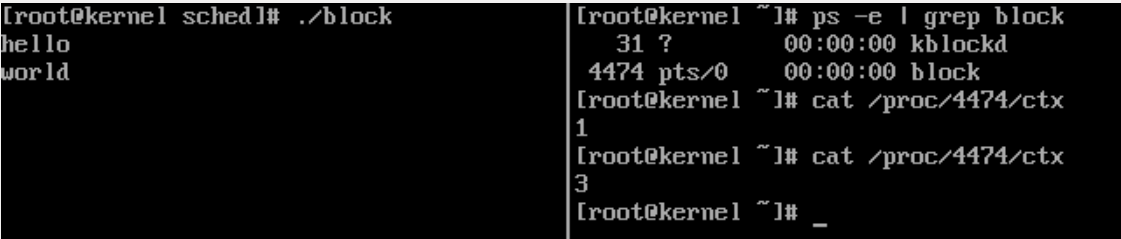
\includegraphics[width=12cm]{sched.png}
\caption{Demo of the scheduler counter}
\end{figure}
As we can see here, when the program is first loaded into memory, it get scheduled to CPU once. Then we typed two lines of text to it and we can find that the {\tt ctx} counter goes up to 3, which is the expected result.

\section{Bonus Part: {\tt top} for {\tt ctx}}
One bonus part of this project is to implement a program that behaves like the Linux command {\tt top}. This can be easily done by interacting with proc file system. In this project, I simply use Python to do this since Python is a quite handy script programming language, which means that we can do formatting and interact with file system easily.

To make the program display the real-time information of the scheduler counter, we can use the Linux library \emph{curses}. This library can make the display in console much easier and we can repaint the console as we want. The source code is shown as follows:
\begin{lstlisting}[language=python, caption=top for ctx]
import os, time, curses

def get_info():
	dirs = [s for s in os.listdir('/proc') if s.isdigit()]
	info = []
	for d in dirs:
		pid = comm = ctx = ''
		pid = d
		with open('/proc/' + d + '/comm') as f:
			comm = f.read().strip('\n')
		with open('/proc/' + d + '/ctx') as f:
			ctx = f.read().strip('\n')
		info.append((pid, comm, ctx))
	return info

def info_to_strs():
	top_info = sorted(get_info(), key=lambda i: int(i[2]), reverse=True)[:20]
	strs = []
	for i in top_info:
		strs.append(i[0].rjust(5) + ' ' + i[1].ljust(15) + i[2].rjust(6))
	return strs


screen = curses.initscr()
screen.keypad(1)
screen.nodelay(1)
curses.noecho()

while (True):
	strs = info_to_strs()
	screen.clear()
	for s in strs:
		screen.addstr(s + "\n")
		screen.refresh()
	key = screen.getch()
	if key == ord('q'):
		break;
	time.sleep(1.0)

curses.endwin()
\end{lstlisting}




\section{Conclusion}

In this project, we mainly deal with the Linux process scheduler. I learned a lot from the Linux's completely fair scheduler and have more hands-on with regard to the proc file system. Also, with the help of Arch Linux, now I have a more compact understanding of the Linux philosophy --- \emph{keep it simple, stupid}.

\section*{Acknowledgement}
Thanks Prof. Chen for guidance on Linux kernel and TAs for their hard work.
\end{document}
